\chapter{Experimenty a vyhodnocení} \label{chap:eval}
  V~navrženém systému byly implementovány a odsimulovány 4 vybrané metody přistávání (\cref{chap:algs}), na nichž byly provedeny experimenty popsané v~této kapitole, které sloužily primárně ke zjištění rozdílů mezi implementovanými algoritmy podle různých hledisek. Během několikrát opakované simulace byly sledovány určité ukazatele, které byly zaznamenávány a statisticky zpracovány, konkrétní provedení je vždy uvedeno v~příslušné podkapitole daného experimentu. Pro provedení experimentů \cref*{sec:presnostPristani,sec:presnostPristavani,sec:uspesnost} bylo zvoleno 5 různých tříd větrných podmínek (bezvětří, slabý vítr, slabý vítr s~poryvy, čerstvý vítr, čerstvý vítr s~poryvy). Nastavení simulačních parametrů v~jednotlivých třídách shrnuje \cref{tab:tridyVetru}.
  \begin{table}[H]
    \centering
    \begin{tabular}{@{}lllll@{}}
      \hline
      třída & $v$ [m/s] & $\sigma_v$ [m/s] & $\varsigma$ [$^{\circ}$] & $\sigma_\varsigma$ [$^{\circ}$] \bigstrut\\
      \hline
      bezvětří & 0     & 0     & 0     & 0 \bigstrut[t]\\
      slabý vítr & 3     & 1     & 105   & 10 \\
      slabý vítr s~poryvy & 3     & 3     & 105   & 20 \\
      čerstvý vítr & 8     & 2     & 105   & 10 \\
      čerstvý vítr s~poryvy & 8     & 4     & 105   & 20 \bigstrut[b]\\
      \hline
      \end{tabular}%
    \caption[Třídy větrných podmínek]{Třídy větrných podmínek a jejich parametry použité při simulaci v~některých experimentech.}
    \label{tab:tridyVetru}
  \end{table}
  \section{Přesnost přistání} \label{sec:presnostPristani}
    % Including files from KAP1
\newcommand{\NstepsMeanKAPILbezvetri}{$613{,}18$}
\newcommand{\NstepsSumKAPILbezvetri}{$3{,}13 \times 10^{4}$}
\newcommand{\NstepsVarKAPILbezvetri}{$75{,}36$}
\newcommand{\NstepsWoVisionMeanKAPILbezvetri}{$0{,}00$}
\newcommand{\NstepsWoVisionVarKAPILbezvetri}{$0{,}00$}
\newcommand{\meanShareWoVisionKAPILbezvetri}{$0{,}00$}
\newcommand{\mistoPristaniXmeanKAPILbezvetri}{$-1{,}22 \times 10^{-3}$}
\newcommand{\mistoPristaniYmeanKAPILbezvetri}{$1{,}18 \times 10^{-3}$}
\newcommand{\mistoPristaniYAWmeanKAPILbezvetri}{$-0{,}11$}
\newcommand{\mistoPristaniXvarKAPILbezvetri}{$2{,}18 \times 10^{-3}$}
\newcommand{\mistoPristaniYvarKAPILbezvetri}{$1{,}40 \times 10^{-4}$}
\newcommand{\mistoPristaniYAWvarKAPILbezvetri}{$23{,}27$}
\newcommand{\mistoPredPristaniXmeanKAPILbezvetri}{$-6{,}92 \times 10^{-3}$}
\newcommand{\mistoPredPristaniYmeanKAPILbezvetri}{$2{,}62 \times 10^{-3}$}
\newcommand{\mistoPredPristaniYAWmeanKAPILbezvetri}{$-0{,}42$}
\newcommand{\mistoPredPristaniXvarKAPILbezvetri}{$2{,}59 \times 10^{-3}$}
\newcommand{\mistoPredPristaniYvarKAPILbezvetri}{$1{,}65 \times 10^{-5}$}
\newcommand{\mistoPredPristaniYAWvarKAPILbezvetri}{$55{,}33$}
\newcommand{\landingRetriesMeanKAPILbezvetri}{$1{,}00$}
\newcommand{\MAExKAPILbezvetri}{$0{,}10$}
\newcommand{\MAEyKAPILbezvetri}{$5{,}70 \times 10^{-2}$}
\newcommand{\MAEyawKAPILbezvetri}{$4{,}19$}
\newcommand{\simDurationMeanKAPILbezvetri}{$55{,}63$}
\newcommand{\simDurationVarKAPILbezvetri}{$0{,}51$}
\newcommand{\RTdurationMeanKAPILbezvetri}{$61{,}03$}
\newcommand{\RTdurationVarKAPILbezvetri}{$3{,}13$}
\newcommand{\RTFmeanKAPILbezvetri}{$0{,}91$}
\newcommand{\RTFvarKAPILbezvetri}{$3{,}83 \times 10^{-4}$}
\newcommand{\meanStepDurationAverageKAPILbezvetri}{$2{,}91 \times 10^{-2}$}
\newcommand{\meanStepDurationVarKAPILbezvetri}{$1{,}34 \times 10^{-5}$}
\newcommand{\landingDurationMeanKAPILbezvetri}{$22{,}90$}
\newcommand{\landingDurationVarKAPILbezvetri}{$0{,}51$}
\newcommand{\sampleSizeKAPILbezvetri}{$51{,}00$}

\newcommand{\NstepsMeanKAPILvitrI}{$615{,}24$}
\newcommand{\NstepsSumKAPILvitrI}{$3{,}08 \times 10^{4}$}
\newcommand{\NstepsVarKAPILvitrI}{$250{,}74$}
\newcommand{\NstepsWoVisionMeanKAPILvitrI}{$0{,}00$}
\newcommand{\NstepsWoVisionVarKAPILvitrI}{$0{,}00$}
\newcommand{\meanShareWoVisionKAPILvitrI}{$0{,}00$}
\newcommand{\mistoPristaniXmeanKAPILvitrI}{$-3{,}54 \times 10^{-2}$}
\newcommand{\mistoPristaniYmeanKAPILvitrI}{$-8{,}62 \times 10^{-2}$}
\newcommand{\mistoPristaniYAWmeanKAPILvitrI}{$-0{,}84$}
\newcommand{\mistoPristaniXvarKAPILvitrI}{$2{,}57 \times 10^{-4}$}
\newcommand{\mistoPristaniYvarKAPILvitrI}{$1{,}62 \times 10^{-3}$}
\newcommand{\mistoPristaniYAWvarKAPILvitrI}{$1{,}09$}
\newcommand{\mistoPredPristaniXmeanKAPILvitrI}{$-1{,}86 \times 10^{-2}$}
\newcommand{\mistoPredPristaniYmeanKAPILvitrI}{$4{,}54 \times 10^{-2}$}
\newcommand{\mistoPredPristaniYAWmeanKAPILvitrI}{$0{,}40$}
\newcommand{\mistoPredPristaniXvarKAPILvitrI}{$2{,}27 \times 10^{-4}$}
\newcommand{\mistoPredPristaniYvarKAPILvitrI}{$6{,}26 \times 10^{-4}$}
\newcommand{\mistoPredPristaniYAWvarKAPILvitrI}{$1{,}27 \times 10^{-2}$}
\newcommand{\landingRetriesMeanKAPILvitrI}{$1{,}00$}
\newcommand{\MAExKAPILvitrI}{$7{,}87 \times 10^{-2}$}
\newcommand{\MAEyKAPILvitrI}{$7{,}75 \times 10^{-2}$}
\newcommand{\MAEyawKAPILvitrI}{$3{,}82$}
\newcommand{\simDurationMeanKAPILvitrI}{$55{,}34$}
\newcommand{\simDurationVarKAPILvitrI}{$0{,}23$}
\newcommand{\RTdurationMeanKAPILvitrI}{$60{,}82$}
\newcommand{\RTdurationVarKAPILvitrI}{$1{,}71$}
\newcommand{\RTFmeanKAPILvitrI}{$0{,}91$}
\newcommand{\RTFvarKAPILvitrI}{$3{,}54 \times 10^{-4}$}
\newcommand{\meanStepDurationAverageKAPILvitrI}{$2{,}95 \times 10^{-2}$}
\newcommand{\meanStepDurationVarKAPILvitrI}{$1{,}32 \times 10^{-5}$}
\newcommand{\landingDurationMeanKAPILvitrI}{$22{,}81$}
\newcommand{\landingDurationVarKAPILvitrI}{$0{,}23$}
\newcommand{\sampleSizeKAPILvitrI}{$50{,}00$}

\newcommand{\NstepsMeanKAPILvitrII}{$653{,}32$}
\newcommand{\NstepsSumKAPILvitrII}{$3{,}27 \times 10^{4}$}
\newcommand{\NstepsVarKAPILvitrII}{$7{,}38 \times 10^{3}$}
\newcommand{\NstepsWoVisionMeanKAPILvitrII}{$6{,}00 \times 10^{-2}$}
\newcommand{\NstepsWoVisionVarKAPILvitrII}{$0{,}18$}
\newcommand{\meanShareWoVisionKAPILvitrII}{$6{,}17 \times 10^{-5}$}
\newcommand{\mistoPristaniXmeanKAPILvitrII}{$-2{,}90 \times 10^{-2}$}
\newcommand{\mistoPristaniYmeanKAPILvitrII}{$-6{,}07 \times 10^{-2}$}
\newcommand{\mistoPristaniYAWmeanKAPILvitrII}{$-0{,}65$}
\newcommand{\mistoPristaniXvarKAPILvitrII}{$2{,}46 \times 10^{-3}$}
\newcommand{\mistoPristaniYvarKAPILvitrII}{$1{,}03 \times 10^{-2}$}
\newcommand{\mistoPristaniYAWvarKAPILvitrII}{$3{,}63$}
\newcommand{\mistoPredPristaniXmeanKAPILvitrII}{$-1{,}85 \times 10^{-2}$}
\newcommand{\mistoPredPristaniYmeanKAPILvitrII}{$5{,}37 \times 10^{-2}$}
\newcommand{\mistoPredPristaniYAWmeanKAPILvitrII}{$0{,}41$}
\newcommand{\mistoPredPristaniXvarKAPILvitrII}{$1{,}76 \times 10^{-3}$}
\newcommand{\mistoPredPristaniYvarKAPILvitrII}{$5{,}35 \times 10^{-3}$}
\newcommand{\mistoPredPristaniYAWvarKAPILvitrII}{$3{,}28$}
\newcommand{\landingRetriesMeanKAPILvitrII}{$1{,}00$}
\newcommand{\MAExKAPILvitrII}{$0{,}10$}
\newcommand{\MAEyKAPILvitrII}{$0{,}11$}
\newcommand{\MAEyawKAPILvitrII}{$4{,}75$}
\newcommand{\simDurationMeanKAPILvitrII}{$56{,}80$}
\newcommand{\simDurationVarKAPILvitrII}{$9{,}30$}
\newcommand{\RTdurationMeanKAPILvitrII}{$63{,}95$}
\newcommand{\RTdurationVarKAPILvitrII}{$27{,}84$}
\newcommand{\RTFmeanKAPILvitrII}{$0{,}89$}
\newcommand{\RTFvarKAPILvitrII}{$9{,}03 \times 10^{-4}$}
\newcommand{\meanStepDurationAverageKAPILvitrII}{$3{,}15 \times 10^{-2}$}
\newcommand{\meanStepDurationVarKAPILvitrII}{$2{,}06 \times 10^{-5}$}
\newcommand{\landingDurationMeanKAPILvitrII}{$24{,}22$}
\newcommand{\landingDurationVarKAPILvitrII}{$9{,}36$}
\newcommand{\sampleSizeKAPILvitrII}{$50{,}00$}

\newcommand{\NstepsMeanKAPILvitrIII}{$739{,}58$}
\newcommand{\NstepsSumKAPILvitrIII}{$3{,}70 \times 10^{4}$}
\newcommand{\NstepsVarKAPILvitrIII}{$4{,}22 \times 10^{4}$}
\newcommand{\NstepsWoVisionMeanKAPILvitrIII}{$30{,}36$}
\newcommand{\NstepsWoVisionVarKAPILvitrIII}{$1{,}45 \times 10^{3}$}
\newcommand{\meanShareWoVisionKAPILvitrIII}{$3{,}47 \times 10^{-2}$}
\newcommand{\mistoPristaniXmeanKAPILvitrIII}{$-7{,}48 \times 10^{-2}$}
\newcommand{\mistoPristaniYmeanKAPILvitrIII}{$-0{,}25$}
\newcommand{\mistoPristaniYAWmeanKAPILvitrIII}{$-0{,}85$}
\newcommand{\mistoPristaniXvarKAPILvitrIII}{$2{,}20 \times 10^{-3}$}
\newcommand{\mistoPristaniYvarKAPILvitrIII}{$9{,}88 \times 10^{-3}$}
\newcommand{\mistoPristaniYAWvarKAPILvitrIII}{$11{,}09$}
\newcommand{\mistoPredPristaniXmeanKAPILvitrIII}{$-3{,}78 \times 10^{-2}$}
\newcommand{\mistoPredPristaniYmeanKAPILvitrIII}{$7{,}19 \times 10^{-2}$}
\newcommand{\mistoPredPristaniYAWmeanKAPILvitrIII}{$1{,}48$}
\newcommand{\mistoPredPristaniXvarKAPILvitrIII}{$1{,}05 \times 10^{-3}$}
\newcommand{\mistoPredPristaniYvarKAPILvitrIII}{$2{,}26 \times 10^{-3}$}
\newcommand{\mistoPredPristaniYAWvarKAPILvitrIII}{$3{,}87 \times 10^{-2}$}
\newcommand{\landingRetriesMeanKAPILvitrIII}{$1{,}10$}
\newcommand{\MAExKAPILvitrIII}{$0{,}11$}
\newcommand{\MAEyKAPILvitrIII}{$0{,}12$}
\newcommand{\MAEyawKAPILvitrIII}{$4{,}07$}
\newcommand{\simDurationMeanKAPILvitrIII}{$60{,}49$}
\newcommand{\simDurationVarKAPILvitrIII}{$81{,}64$}
\newcommand{\RTdurationMeanKAPILvitrIII}{$68{,}42$}
\newcommand{\RTdurationVarKAPILvitrIII}{$140{,}20$}
\newcommand{\RTFmeanKAPILvitrIII}{$0{,}89$}
\newcommand{\RTFvarKAPILvitrIII}{$3{,}88 \times 10^{-3}$}
\newcommand{\meanStepDurationAverageKAPILvitrIII}{$2{,}99 \times 10^{-2}$}
\newcommand{\meanStepDurationVarKAPILvitrIII}{$2{,}00 \times 10^{-5}$}
\newcommand{\landingDurationMeanKAPILvitrIII}{$27{,}76$}
\newcommand{\landingDurationVarKAPILvitrIII}{$80{,}69$}
\newcommand{\sampleSizeKAPILvitrIII}{$50{,}00$}

\newcommand{\NstepsMeanKAPILvitrIV}{$821{,}48$}
\newcommand{\NstepsSumKAPILvitrIV}{$4{,}11 \times 10^{4}$}
\newcommand{\NstepsVarKAPILvitrIV}{$1{,}74 \times 10^{5}$}
\newcommand{\NstepsWoVisionMeanKAPILvitrIV}{$27{,}56$}
\newcommand{\NstepsWoVisionVarKAPILvitrIV}{$2{,}01 \times 10^{3}$}
\newcommand{\meanShareWoVisionKAPILvitrIV}{$2{,}37 \times 10^{-2}$}
\newcommand{\mistoPristaniXmeanKAPILvitrIV}{$-3{,}12 \times 10^{-2}$}
\newcommand{\mistoPristaniYmeanKAPILvitrIV}{$-0{,}27$}
\newcommand{\mistoPristaniYAWmeanKAPILvitrIV}{$-1{,}03$}
\newcommand{\mistoPristaniXvarKAPILvitrIV}{$3{,}79 \times 10^{-3}$}
\newcommand{\mistoPristaniYvarKAPILvitrIV}{$1{,}38 \times 10^{-2}$}
\newcommand{\mistoPristaniYAWvarKAPILvitrIV}{$28{,}33$}
\newcommand{\mistoPredPristaniXmeanKAPILvitrIV}{$9{,}76 \times 10^{-3}$}
\newcommand{\mistoPredPristaniYmeanKAPILvitrIV}{$1{,}09 \times 10^{-2}$}
\newcommand{\mistoPredPristaniYAWmeanKAPILvitrIV}{$1{,}40$}
\newcommand{\mistoPredPristaniXvarKAPILvitrIV}{$2{,}83 \times 10^{-3}$}
\newcommand{\mistoPredPristaniYvarKAPILvitrIV}{$6{,}04 \times 10^{-3}$}
\newcommand{\mistoPredPristaniYAWvarKAPILvitrIV}{$8{,}48 \times 10^{-2}$}
\newcommand{\landingRetriesMeanKAPILvitrIV}{$1{,}26$}
\newcommand{\MAExKAPILvitrIV}{$0{,}11$}
\newcommand{\MAEyKAPILvitrIV}{$0{,}13$}
\newcommand{\MAEyawKAPILvitrIV}{$4{,}10$}
\newcommand{\simDurationMeanKAPILvitrIV}{$64{,}17$}
\newcommand{\simDurationVarKAPILvitrIV}{$350{,}02$}
\newcommand{\RTdurationMeanKAPILvitrIV}{$71{,}56$}
\newcommand{\RTdurationVarKAPILvitrIV}{$503{,}27$}
\newcommand{\RTFmeanKAPILvitrIV}{$0{,}90$}
\newcommand{\RTFvarKAPILvitrIV}{$5{,}04 \times 10^{-4}$}
\newcommand{\meanStepDurationAverageKAPILvitrIV}{$2{,}79 \times 10^{-2}$}
\newcommand{\meanStepDurationVarKAPILvitrIV}{$7{,}28 \times 10^{-6}$}
\newcommand{\landingDurationMeanKAPILvitrIV}{$31{,}70$}
\newcommand{\landingDurationVarKAPILvitrIV}{$349{,}59$}
\newcommand{\sampleSizeKAPILvitrIV}{$50{,}00$}


% Including files from K_P1
\newcommand{\NstepsMeanKLPILbezvetri}{$596{,}88$}
\newcommand{\NstepsSumKLPILbezvetri}{$2{,}98 \times 10^{4}$}
\newcommand{\NstepsVarKLPILbezvetri}{$1{,}87$}
\newcommand{\NstepsWoVisionMeanKLPILbezvetri}{$0{,}00$}
\newcommand{\NstepsWoVisionVarKLPILbezvetri}{$0{,}00$}
\newcommand{\meanShareWoVisionKLPILbezvetri}{$0{,}00$}
\newcommand{\mistoPristaniXmeanKLPILbezvetri}{$1{,}66 \times 10^{-3}$}
\newcommand{\mistoPristaniYmeanKLPILbezvetri}{$4{,}87 \times 10^{-3}$}
\newcommand{\mistoPristaniYAWmeanKLPILbezvetri}{$0{,}20$}
\newcommand{\mistoPristaniXvarKLPILbezvetri}{$4{,}84 \times 10^{-5}$}
\newcommand{\mistoPristaniYvarKLPILbezvetri}{$4{,}66 \times 10^{-4}$}
\newcommand{\mistoPristaniYAWvarKLPILbezvetri}{$3{,}28 \times 10^{-3}$}
\newcommand{\mistoPredPristaniXmeanKLPILbezvetri}{$3{,}53 \times 10^{-3}$}
\newcommand{\mistoPredPristaniYmeanKLPILbezvetri}{$-5{,}55 \times 10^{-4}$}
\newcommand{\mistoPredPristaniYAWmeanKLPILbezvetri}{$0{,}18$}
\newcommand{\mistoPredPristaniXvarKLPILbezvetri}{$3{,}64 \times 10^{-6}$}
\newcommand{\mistoPredPristaniYvarKLPILbezvetri}{$2{,}80 \times 10^{-6}$}
\newcommand{\mistoPredPristaniYAWvarKLPILbezvetri}{$6{,}52 \times 10^{-5}$}
\newcommand{\landingRetriesMeanKLPILbezvetri}{$1{,}00$}
\newcommand{\MAExKLPILbezvetri}{$0{,}10$}
\newcommand{\MAEyKLPILbezvetri}{$5{,}23 \times 10^{-2}$}
\newcommand{\MAEyawKLPILbezvetri}{$3{,}72$}
\newcommand{\simDurationMeanKLPILbezvetri}{$49{,}15$}
\newcommand{\simDurationVarKLPILbezvetri}{$0{,}12$}
\newcommand{\RTdurationMeanKLPILbezvetri}{$54{,}52$}
\newcommand{\RTdurationVarKLPILbezvetri}{$1{,}57$}
\newcommand{\RTFmeanKLPILbezvetri}{$0{,}90$}
\newcommand{\RTFvarKLPILbezvetri}{$3{,}78 \times 10^{-4}$}
\newcommand{\meanStepDurationAverageKLPILbezvetri}{$2{,}61 \times 10^{-2}$}
\newcommand{\meanStepDurationVarKLPILbezvetri}{$5{,}84 \times 10^{-6}$}
\newcommand{\landingDurationMeanKLPILbezvetri}{$22{,}41$}
\newcommand{\landingDurationVarKLPILbezvetri}{$0{,}11$}
\newcommand{\sampleSizeKLPILbezvetri}{$50{,}00$}

\newcommand{\NstepsMeanKLPILvitrI}{$602{,}40$}
\newcommand{\NstepsSumKLPILvitrI}{$3{,}01 \times 10^{4}$}
\newcommand{\NstepsVarKLPILvitrI}{$3{,}04$}
\newcommand{\NstepsWoVisionMeanKLPILvitrI}{$0{,}00$}
\newcommand{\NstepsWoVisionVarKLPILvitrI}{$0{,}00$}
\newcommand{\meanShareWoVisionKLPILvitrI}{$0{,}00$}
\newcommand{\mistoPristaniXmeanKLPILvitrI}{$-1{,}89 \times 10^{-2}$}
\newcommand{\mistoPristaniYmeanKLPILvitrI}{$-0{,}14$}
\newcommand{\mistoPristaniYAWmeanKLPILvitrI}{$-0{,}53$}
\newcommand{\mistoPristaniXvarKLPILvitrI}{$2{,}42 \times 10^{-4}$}
\newcommand{\mistoPristaniYvarKLPILvitrI}{$2{,}35 \times 10^{-3}$}
\newcommand{\mistoPristaniYAWvarKLPILvitrI}{$1{,}06$}
\newcommand{\mistoPredPristaniXmeanKLPILvitrI}{$4{,}21 \times 10^{-4}$}
\newcommand{\mistoPredPristaniYmeanKLPILvitrI}{$-1{,}94 \times 10^{-2}$}
\newcommand{\mistoPredPristaniYAWmeanKLPILvitrI}{$0{,}39$}
\newcommand{\mistoPredPristaniXvarKLPILvitrI}{$2{,}49 \times 10^{-4}$}
\newcommand{\mistoPredPristaniYvarKLPILvitrI}{$3{,}93 \times 10^{-4}$}
\newcommand{\mistoPredPristaniYAWvarKLPILvitrI}{$1{,}59 \times 10^{-3}$}
\newcommand{\landingRetriesMeanKLPILvitrI}{$1{,}00$}
\newcommand{\MAExKLPILvitrI}{$8{,}80 \times 10^{-2}$}
\newcommand{\MAEyKLPILvitrI}{$0{,}09$}
\newcommand{\MAEyawKLPILvitrI}{$3{,}75$}
\newcommand{\simDurationMeanKLPILvitrI}{$49{,}21$}
\newcommand{\simDurationVarKLPILvitrI}{$0{,}16$}
\newcommand{\RTdurationMeanKLPILvitrI}{$54{,}36$}
\newcommand{\RTdurationVarKLPILvitrI}{$1{,}18$}
\newcommand{\RTFmeanKLPILvitrI}{$0{,}91$}
\newcommand{\RTFvarKLPILvitrI}{$3{,}51 \times 10^{-4}$}
\newcommand{\meanStepDurationAverageKLPILvitrI}{$2{,}55 \times 10^{-2}$}
\newcommand{\meanStepDurationVarKLPILvitrI}{$4{,}89 \times 10^{-6}$}
\newcommand{\landingDurationMeanKLPILvitrI}{$22{,}39$}
\newcommand{\landingDurationVarKLPILvitrI}{$0{,}16$}
\newcommand{\sampleSizeKLPILvitrI}{$50{,}00$}

\newcommand{\NstepsMeanKLPILvitrII}{$613{,}64$}
\newcommand{\NstepsSumKLPILvitrII}{$3{,}07 \times 10^{4}$}
\newcommand{\NstepsVarKLPILvitrII}{$37{,}35$}
\newcommand{\NstepsWoVisionMeanKLPILvitrII}{$4{,}00 \times 10^{-2}$}
\newcommand{\NstepsWoVisionVarKLPILvitrII}{$7{,}84 \times 10^{-2}$}
\newcommand{\meanShareWoVisionKLPILvitrII}{$6{,}43 \times 10^{-5}$}
\newcommand{\mistoPristaniXmeanKLPILvitrII}{$-3{,}17 \times 10^{-2}$}
\newcommand{\mistoPristaniYmeanKLPILvitrII}{$-0{,}14$}
\newcommand{\mistoPristaniYAWmeanKLPILvitrII}{$-0{,}82$}
\newcommand{\mistoPristaniXvarKLPILvitrII}{$1{,}13 \times 10^{-3}$}
\newcommand{\mistoPristaniYvarKLPILvitrII}{$6{,}02 \times 10^{-3}$}
\newcommand{\mistoPristaniYAWvarKLPILvitrII}{$2{,}05$}
\newcommand{\mistoPredPristaniXmeanKLPILvitrII}{$-8{,}72 \times 10^{-3}$}
\newcommand{\mistoPredPristaniYmeanKLPILvitrII}{$-1{,}75 \times 10^{-2}$}
\newcommand{\mistoPredPristaniYAWmeanKLPILvitrII}{$0{,}36$}
\newcommand{\mistoPredPristaniXvarKLPILvitrII}{$9{,}24 \times 10^{-4}$}
\newcommand{\mistoPredPristaniYvarKLPILvitrII}{$3{,}12 \times 10^{-3}$}
\newcommand{\mistoPredPristaniYAWvarKLPILvitrII}{$5{,}42 \times 10^{-3}$}
\newcommand{\landingRetriesMeanKLPILvitrII}{$1{,}00$}
\newcommand{\MAExKLPILvitrII}{$0{,}10$}
\newcommand{\MAEyKLPILvitrII}{$0{,}11$}
\newcommand{\MAEyawKLPILvitrII}{$3{,}65$}
\newcommand{\simDurationMeanKLPILvitrII}{$49{,}63$}
\newcommand{\simDurationVarKLPILvitrII}{$0{,}28$}
\newcommand{\RTdurationMeanKLPILvitrII}{$54{,}81$}
\newcommand{\RTdurationVarKLPILvitrII}{$1{,}48$}
\newcommand{\RTFmeanKLPILvitrII}{$0{,}91$}
\newcommand{\RTFvarKLPILvitrII}{$3{,}04 \times 10^{-4}$}
\newcommand{\meanStepDurationAverageKLPILvitrII}{$2{,}52 \times 10^{-2}$}
\newcommand{\meanStepDurationVarKLPILvitrII}{$4{,}81 \times 10^{-6}$}
\newcommand{\landingDurationMeanKLPILvitrII}{$22{,}85$}
\newcommand{\landingDurationVarKLPILvitrII}{$0{,}25$}
\newcommand{\sampleSizeKLPILvitrII}{$50{,}00$}

\newcommand{\NstepsMeanKLPILvitrIII}{$965{,}72$}
\newcommand{\NstepsSumKLPILvitrIII}{$4{,}83 \times 10^{4}$}
\newcommand{\NstepsVarKLPILvitrIII}{$2{,}28 \times 10^{5}$}
\newcommand{\NstepsWoVisionMeanKLPILvitrIII}{$122{,}74$}
\newcommand{\NstepsWoVisionVarKLPILvitrIII}{$2{,}55 \times 10^{4}$}
\newcommand{\meanShareWoVisionKLPILvitrIII}{$8{,}96 \times 10^{-2}$}
\newcommand{\mistoPristaniXmeanKLPILvitrIII}{$-5{,}24 \times 10^{-2}$}
\newcommand{\mistoPristaniYmeanKLPILvitrIII}{$-0{,}38$}
\newcommand{\mistoPristaniYAWmeanKLPILvitrIII}{$0{,}86$}
\newcommand{\mistoPristaniXvarKLPILvitrIII}{$1{,}67 \times 10^{-3}$}
\newcommand{\mistoPristaniYvarKLPILvitrIII}{$9{,}83 \times 10^{-3}$}
\newcommand{\mistoPristaniYAWvarKLPILvitrIII}{$11{,}90$}
\newcommand{\mistoPredPristaniXmeanKLPILvitrIII}{$6{,}23 \times 10^{-3}$}
\newcommand{\mistoPredPristaniYmeanKLPILvitrIII}{$-2{,}07 \times 10^{-2}$}
\newcommand{\mistoPredPristaniYAWmeanKLPILvitrIII}{$1{,}45$}
\newcommand{\mistoPredPristaniXvarKLPILvitrIII}{$1{,}09 \times 10^{-3}$}
\newcommand{\mistoPredPristaniYvarKLPILvitrIII}{$7{,}29 \times 10^{-4}$}
\newcommand{\mistoPredPristaniYAWvarKLPILvitrIII}{$0{,}14$}
\newcommand{\landingRetriesMeanKLPILvitrIII}{$2{,}16$}
\newcommand{\MAExKLPILvitrIII}{$0{,}11$}
\newcommand{\MAEyKLPILvitrIII}{$0{,}18$}
\newcommand{\MAEyawKLPILvitrIII}{$3{,}72$}
\newcommand{\simDurationMeanKLPILvitrIII}{$66{,}81$}
\newcommand{\simDurationVarKLPILvitrIII}{$629{,}78$}
\newcommand{\RTdurationMeanKLPILvitrIII}{$73{,}47$}
\newcommand{\RTdurationVarKLPILvitrIII}{$711{,}71$}
\newcommand{\RTFmeanKLPILvitrIII}{$0{,}91$}
\newcommand{\RTFvarKLPILvitrIII}{$3{,}58 \times 10^{-4}$}
\newcommand{\meanStepDurationAverageKLPILvitrIII}{$2{,}38 \times 10^{-2}$}
\newcommand{\meanStepDurationVarKLPILvitrIII}{$5{,}56 \times 10^{-6}$}
\newcommand{\landingDurationMeanKLPILvitrIII}{$39{,}93$}
\newcommand{\landingDurationVarKLPILvitrIII}{$628{,}40$}
\newcommand{\sampleSizeKLPILvitrIII}{$50{,}00$}

\newcommand{\NstepsMeanKLPILvitrIV}{$1{,}03 \times 10^{3}$}
\newcommand{\NstepsSumKLPILvitrIV}{$5{,}13 \times 10^{4}$}
\newcommand{\NstepsVarKLPILvitrIV}{$2{,}18 \times 10^{5}$}
\newcommand{\NstepsWoVisionMeanKLPILvitrIV}{$138{,}80$}
\newcommand{\NstepsWoVisionVarKLPILvitrIV}{$2{,}83 \times 10^{4}$}
\newcommand{\meanShareWoVisionKLPILvitrIV}{$0{,}09$}
\newcommand{\mistoPristaniXmeanKLPILvitrIV}{$-4{,}80 \times 10^{-2}$}
\newcommand{\mistoPristaniYmeanKLPILvitrIV}{$-0{,}34$}
\newcommand{\mistoPristaniYAWmeanKLPILvitrIV}{$1{,}39$}
\newcommand{\mistoPristaniXvarKLPILvitrIV}{$3{,}81 \times 10^{-3}$}
\newcommand{\mistoPristaniYvarKLPILvitrIV}{$1{,}42 \times 10^{-2}$}
\newcommand{\mistoPristaniYAWvarKLPILvitrIV}{$15{,}35$}
\newcommand{\mistoPredPristaniXmeanKLPILvitrIV}{$1{,}60 \times 10^{-2}$}
\newcommand{\mistoPredPristaniYmeanKLPILvitrIV}{$3{,}96 \times 10^{-3}$}
\newcommand{\mistoPredPristaniYAWmeanKLPILvitrIV}{$1{,}46$}
\newcommand{\mistoPredPristaniXvarKLPILvitrIV}{$3{,}25 \times 10^{-3}$}
\newcommand{\mistoPredPristaniYvarKLPILvitrIV}{$2{,}04 \times 10^{-3}$}
\newcommand{\mistoPredPristaniYAWvarKLPILvitrIV}{$0{,}14$}
\newcommand{\landingRetriesMeanKLPILvitrIV}{$2{,}42$}
\newcommand{\MAExKLPILvitrIV}{$0{,}12$}
\newcommand{\MAEyKLPILvitrIV}{$0{,}17$}
\newcommand{\MAEyawKLPILvitrIV}{$3{,}66$}
\newcommand{\simDurationMeanKLPILvitrIV}{$69{,}84$}
\newcommand{\simDurationVarKLPILvitrIV}{$588{,}52$}
\newcommand{\RTdurationMeanKLPILvitrIV}{$76{,}86$}
\newcommand{\RTdurationVarKLPILvitrIV}{$717{,}28$}
\newcommand{\RTFmeanKLPILvitrIV}{$0{,}91$}
\newcommand{\RTFvarKLPILvitrIV}{$3{,}19 \times 10^{-4}$}
\newcommand{\meanStepDurationAverageKLPILvitrIV}{$2{,}39 \times 10^{-2}$}
\newcommand{\meanStepDurationVarKLPILvitrIV}{$4{,}08 \times 10^{-6}$}
\newcommand{\landingDurationMeanKLPILvitrIV}{$42{,}97$}
\newcommand{\landingDurationVarKLPILvitrIV}{$589{,}15$}
\newcommand{\sampleSizeKLPILvitrIV}{$50{,}00$}


% Including files from _AP1
\newcommand{\NstepsMeanLAPILbezvetri}{$594{,}34$}
\newcommand{\NstepsSumLAPILbezvetri}{$2{,}97 \times 10^{4}$}
\newcommand{\NstepsVarLAPILbezvetri}{$2{,}78$}
\newcommand{\NstepsWoVisionMeanLAPILbezvetri}{$0{,}00$}
\newcommand{\NstepsWoVisionVarLAPILbezvetri}{$0{,}00$}
\newcommand{\meanShareWoVisionLAPILbezvetri}{$0{,}00$}
\newcommand{\mistoPristaniXmeanLAPILbezvetri}{$3{,}11 \times 10^{-3}$}
\newcommand{\mistoPristaniYmeanLAPILbezvetri}{$2{,}00 \times 10^{-3}$}
\newcommand{\mistoPristaniYAWmeanLAPILbezvetri}{$0{,}23$}
\newcommand{\mistoPristaniXvarLAPILbezvetri}{$1{,}53 \times 10^{-5}$}
\newcommand{\mistoPristaniYvarLAPILbezvetri}{$1{,}54 \times 10^{-4}$}
\newcommand{\mistoPristaniYAWvarLAPILbezvetri}{$2{,}28 \times 10^{-2}$}
\newcommand{\mistoPredPristaniXmeanLAPILbezvetri}{$-2{,}03 \times 10^{-3}$}
\newcommand{\mistoPredPristaniYmeanLAPILbezvetri}{$1{,}35 \times 10^{-3}$}
\newcommand{\mistoPredPristaniYAWmeanLAPILbezvetri}{$0{,}19$}
\newcommand{\mistoPredPristaniXvarLAPILbezvetri}{$5{,}23 \times 10^{-6}$}
\newcommand{\mistoPredPristaniYvarLAPILbezvetri}{$8{,}96 \times 10^{-6}$}
\newcommand{\mistoPredPristaniYAWvarLAPILbezvetri}{$3{,}44 \times 10^{-5}$}
\newcommand{\landingRetriesMeanLAPILbezvetri}{$1{,}00$}
\newcommand{\MAExLAPILbezvetri}{$0{,}10$}
\newcommand{\MAEyLAPILbezvetri}{$4{,}46 \times 10^{-2}$}
\newcommand{\MAEyawLAPILbezvetri}{$2{,}48$}
\newcommand{\simDurationMeanLAPILbezvetri}{$55{,}23$}
\newcommand{\simDurationVarLAPILbezvetri}{$0{,}17$}
\newcommand{\RTdurationMeanLAPILbezvetri}{$56{,}85$}
\newcommand{\RTdurationVarLAPILbezvetri}{$0{,}23$}
\newcommand{\RTFmeanLAPILbezvetri}{$0{,}97$}
\newcommand{\RTFvarLAPILbezvetri}{$1{,}24 \times 10^{-5}$}
\newcommand{\meanStepDurationAverageLAPILbezvetri}{$1{,}44 \times 10^{-2}$}
\newcommand{\meanStepDurationVarLAPILbezvetri}{$1{,}63 \times 10^{-6}$}
\newcommand{\landingDurationMeanLAPILbezvetri}{$22{,}52$}
\newcommand{\landingDurationVarLAPILbezvetri}{$0{,}13$}
\newcommand{\sampleSizeLAPILbezvetri}{$50{,}00$}

\newcommand{\NstepsMeanLAPILvitrI}{$592{,}24$}
\newcommand{\NstepsSumLAPILvitrI}{$2{,}96 \times 10^{4}$}
\newcommand{\NstepsVarLAPILvitrI}{$3{,}70$}
\newcommand{\NstepsWoVisionMeanLAPILvitrI}{$0{,}00$}
\newcommand{\NstepsWoVisionVarLAPILvitrI}{$0{,}00$}
\newcommand{\meanShareWoVisionLAPILvitrI}{$0{,}00$}
\newcommand{\mistoPristaniXmeanLAPILvitrI}{$-2{,}59 \times 10^{-2}$}
\newcommand{\mistoPristaniYmeanLAPILvitrI}{$-0{,}12$}
\newcommand{\mistoPristaniYAWmeanLAPILvitrI}{$-0{,}67$}
\newcommand{\mistoPristaniXvarLAPILvitrI}{$2{,}44 \times 10^{-4}$}
\newcommand{\mistoPristaniYvarLAPILvitrI}{$1{,}78 \times 10^{-3}$}
\newcommand{\mistoPristaniYAWvarLAPILvitrI}{$1{,}46$}
\newcommand{\mistoPredPristaniXmeanLAPILvitrI}{$-7{,}50 \times 10^{-3}$}
\newcommand{\mistoPredPristaniYmeanLAPILvitrI}{$5{,}14 \times 10^{-3}$}
\newcommand{\mistoPredPristaniYAWmeanLAPILvitrI}{$0{,}38$}
\newcommand{\mistoPredPristaniXvarLAPILvitrI}{$1{,}25 \times 10^{-4}$}
\newcommand{\mistoPredPristaniYvarLAPILvitrI}{$2{,}30 \times 10^{-4}$}
\newcommand{\mistoPredPristaniYAWvarLAPILvitrI}{$3{,}37 \times 10^{-4}$}
\newcommand{\landingRetriesMeanLAPILvitrI}{$1{,}00$}
\newcommand{\MAExLAPILvitrI}{$8{,}00 \times 10^{-2}$}
\newcommand{\MAEyLAPILvitrI}{$4{,}88 \times 10^{-2}$}
\newcommand{\MAEyawLAPILvitrI}{$2{,}59$}
\newcommand{\simDurationMeanLAPILvitrI}{$54{,}55$}
\newcommand{\simDurationVarLAPILvitrI}{$0{,}25$}
\newcommand{\RTdurationMeanLAPILvitrI}{$56{,}25$}
\newcommand{\RTdurationVarLAPILvitrI}{$0{,}28$}
\newcommand{\RTFmeanLAPILvitrI}{$0{,}97$}
\newcommand{\RTFvarLAPILvitrI}{$1{,}29 \times 10^{-5}$}
\newcommand{\meanStepDurationAverageLAPILvitrI}{$1{,}43 \times 10^{-2}$}
\newcommand{\meanStepDurationVarLAPILvitrI}{$1{,}37 \times 10^{-6}$}
\newcommand{\landingDurationMeanLAPILvitrI}{$21{,}97$}
\newcommand{\landingDurationVarLAPILvitrI}{$0{,}21$}
\newcommand{\sampleSizeLAPILvitrI}{$50{,}00$}

\newcommand{\NstepsMeanLAPILvitrII}{$602{,}52$}
\newcommand{\NstepsSumLAPILvitrII}{$3{,}01 \times 10^{4}$}
\newcommand{\NstepsVarLAPILvitrII}{$31{,}57$}
\newcommand{\NstepsWoVisionMeanLAPILvitrII}{$0{,}00$}
\newcommand{\NstepsWoVisionVarLAPILvitrII}{$0{,}00$}
\newcommand{\meanShareWoVisionLAPILvitrII}{$0{,}00$}
\newcommand{\mistoPristaniXmeanLAPILvitrII}{$-3{,}09 \times 10^{-2}$}
\newcommand{\mistoPristaniYmeanLAPILvitrII}{$-0{,}12$}
\newcommand{\mistoPristaniYAWmeanLAPILvitrII}{$-1{,}10$}
\newcommand{\mistoPristaniXvarLAPILvitrII}{$1{,}73 \times 10^{-3}$}
\newcommand{\mistoPristaniYvarLAPILvitrII}{$5{,}06 \times 10^{-3}$}
\newcommand{\mistoPristaniYAWvarLAPILvitrII}{$2{,}08$}
\newcommand{\mistoPredPristaniXmeanLAPILvitrII}{$-1{,}14 \times 10^{-2}$}
\newcommand{\mistoPredPristaniYmeanLAPILvitrII}{$-1{,}73 \times 10^{-3}$}
\newcommand{\mistoPredPristaniYAWmeanLAPILvitrII}{$0{,}35$}
\newcommand{\mistoPredPristaniXvarLAPILvitrII}{$1{,}62 \times 10^{-3}$}
\newcommand{\mistoPredPristaniYvarLAPILvitrII}{$2{,}95 \times 10^{-3}$}
\newcommand{\mistoPredPristaniYAWvarLAPILvitrII}{$2{,}20 \times 10^{-3}$}
\newcommand{\landingRetriesMeanLAPILvitrII}{$1{,}00$}
\newcommand{\MAExLAPILvitrII}{$8{,}95 \times 10^{-2}$}
\newcommand{\MAEyLAPILvitrII}{$7{,}58 \times 10^{-2}$}
\newcommand{\MAEyawLAPILvitrII}{$2{,}53$}
\newcommand{\simDurationMeanLAPILvitrII}{$55{,}18$}
\newcommand{\simDurationVarLAPILvitrII}{$0{,}30$}
\newcommand{\RTdurationMeanLAPILvitrII}{$56{,}98$}
\newcommand{\RTdurationVarLAPILvitrII}{$0{,}34$}
\newcommand{\RTFmeanLAPILvitrII}{$0{,}97$}
\newcommand{\RTFvarLAPILvitrII}{$2{,}09 \times 10^{-5}$}
\newcommand{\meanStepDurationAverageLAPILvitrII}{$1{,}47 \times 10^{-2}$}
\newcommand{\meanStepDurationVarLAPILvitrII}{$2{,}64 \times 10^{-6}$}
\newcommand{\landingDurationMeanLAPILvitrII}{$22{,}56$}
\newcommand{\landingDurationVarLAPILvitrII}{$0{,}30$}
\newcommand{\sampleSizeLAPILvitrII}{$50{,}00$}

\newcommand{\NstepsMeanLAPILvitrIII}{$621{,}38$}
\newcommand{\NstepsSumLAPILvitrIII}{$3{,}11 \times 10^{4}$}
\newcommand{\NstepsVarLAPILvitrIII}{$154{,}12$}
\newcommand{\NstepsWoVisionMeanLAPILvitrIII}{$7{,}86$}
\newcommand{\NstepsWoVisionVarLAPILvitrIII}{$33{,}76$}
\newcommand{\meanShareWoVisionLAPILvitrIII}{$1{,}25 \times 10^{-2}$}
\newcommand{\mistoPristaniXmeanLAPILvitrIII}{$-4{,}87 \times 10^{-2}$}
\newcommand{\mistoPristaniYmeanLAPILvitrIII}{$-0{,}36$}
\newcommand{\mistoPristaniYAWmeanLAPILvitrIII}{$-1{,}04$}
\newcommand{\mistoPristaniXvarLAPILvitrIII}{$1{,}13 \times 10^{-3}$}
\newcommand{\mistoPristaniYvarLAPILvitrIII}{$8{,}27 \times 10^{-3}$}
\newcommand{\mistoPristaniYAWvarLAPILvitrIII}{$9{,}87$}
\newcommand{\mistoPredPristaniXmeanLAPILvitrIII}{$-5{,}42 \times 10^{-3}$}
\newcommand{\mistoPredPristaniYmeanLAPILvitrIII}{$-2{,}74 \times 10^{-2}$}
\newcommand{\mistoPredPristaniYAWmeanLAPILvitrIII}{$1{,}47$}
\newcommand{\mistoPredPristaniXvarLAPILvitrIII}{$6{,}59 \times 10^{-4}$}
\newcommand{\mistoPredPristaniYvarLAPILvitrIII}{$1{,}48 \times 10^{-3}$}
\newcommand{\mistoPredPristaniYAWvarLAPILvitrIII}{$6{,}64 \times 10^{-3}$}
\newcommand{\landingRetriesMeanLAPILvitrIII}{$1{,}00$}
\newcommand{\MAExLAPILvitrIII}{$7{,}66 \times 10^{-2}$}
\newcommand{\MAEyLAPILvitrIII}{$7{,}57 \times 10^{-2}$}
\newcommand{\MAEyawLAPILvitrIII}{$3{,}33$}
\newcommand{\simDurationMeanLAPILvitrIII}{$55{,}57$}
\newcommand{\simDurationVarLAPILvitrIII}{$0{,}52$}
\newcommand{\RTdurationMeanLAPILvitrIII}{$57{,}48$}
\newcommand{\RTdurationVarLAPILvitrIII}{$0{,}70$}
\newcommand{\RTFmeanLAPILvitrIII}{$0{,}97$}
\newcommand{\RTFvarLAPILvitrIII}{$3{,}60 \times 10^{-5}$}
\newcommand{\meanStepDurationAverageLAPILvitrIII}{$1{,}58 \times 10^{-2}$}
\newcommand{\meanStepDurationVarLAPILvitrIII}{$3{,}69 \times 10^{-6}$}
\newcommand{\landingDurationMeanLAPILvitrIII}{$23{,}10$}
\newcommand{\landingDurationVarLAPILvitrIII}{$0{,}47$}
\newcommand{\sampleSizeLAPILvitrIII}{$50{,}00$}

\newcommand{\NstepsMeanLAPILvitrIV}{$713{,}46$}
\newcommand{\NstepsSumLAPILvitrIV}{$3{,}57 \times 10^{4}$}
\newcommand{\NstepsVarLAPILvitrIV}{$7{,}56 \times 10^{4}$}
\newcommand{\NstepsWoVisionMeanLAPILvitrIV}{$19{,}20$}
\newcommand{\NstepsWoVisionVarLAPILvitrIV}{$1{,}75 \times 10^{3}$}
\newcommand{\meanShareWoVisionLAPILvitrIV}{$1{,}85 \times 10^{-2}$}
\newcommand{\mistoPristaniXmeanLAPILvitrIV}{$-5{,}39 \times 10^{-2}$}
\newcommand{\mistoPristaniYmeanLAPILvitrIV}{$-0{,}29$}
\newcommand{\mistoPristaniYAWmeanLAPILvitrIV}{$0{,}18$}
\newcommand{\mistoPristaniXvarLAPILvitrIV}{$3{,}66 \times 10^{-3}$}
\newcommand{\mistoPristaniYvarLAPILvitrIV}{$1{,}29 \times 10^{-2}$}
\newcommand{\mistoPristaniYAWvarLAPILvitrIV}{$13{,}14$}
\newcommand{\mistoPredPristaniXmeanLAPILvitrIV}{$3{,}97 \times 10^{-3}$}
\newcommand{\mistoPredPristaniYmeanLAPILvitrIV}{$-1{,}16 \times 10^{-2}$}
\newcommand{\mistoPredPristaniYAWmeanLAPILvitrIV}{$1{,}37$}
\newcommand{\mistoPredPristaniXvarLAPILvitrIV}{$2{,}66 \times 10^{-3}$}
\newcommand{\mistoPredPristaniYvarLAPILvitrIV}{$4{,}00 \times 10^{-3}$}
\newcommand{\mistoPredPristaniYAWvarLAPILvitrIV}{$2{,}06 \times 10^{-2}$}
\newcommand{\landingRetriesMeanLAPILvitrIV}{$1{,}12$}
\newcommand{\MAExLAPILvitrIV}{$0{,}09$}
\newcommand{\MAEyLAPILvitrIV}{$0{,}11$}
\newcommand{\MAEyawLAPILvitrIV}{$3{,}23$}
\newcommand{\simDurationMeanLAPILvitrIV}{$59{,}53$}
\newcommand{\simDurationVarLAPILvitrIV}{$142{,}52$}
\newcommand{\RTdurationMeanLAPILvitrIV}{$61{,}38$}
\newcommand{\RTdurationVarLAPILvitrIV}{$150{,}21$}
\newcommand{\RTFmeanLAPILvitrIV}{$0{,}97$}
\newcommand{\RTFvarLAPILvitrIV}{$1{,}18 \times 10^{-5}$}
\newcommand{\meanStepDurationAverageLAPILvitrIV}{$1{,}50 \times 10^{-2}$}
\newcommand{\meanStepDurationVarLAPILvitrIV}{$1{,}69 \times 10^{-6}$}
\newcommand{\landingDurationMeanLAPILvitrIV}{$27{,}00$}
\newcommand{\landingDurationVarLAPILvitrIV}{$143{,}04$}
\newcommand{\sampleSizeLAPILvitrIV}{$50{,}00$}


% Including files from __P1
\newcommand{\NstepsMeanLLPILbezvetri}{$593{,}70$}
\newcommand{\NstepsSumLLPILbezvetri}{$2{,}97 \times 10^{4}$}
\newcommand{\NstepsVarLLPILbezvetri}{$1{,}65$}
\newcommand{\NstepsWoVisionMeanLLPILbezvetri}{$0{,}00$}
\newcommand{\NstepsWoVisionVarLLPILbezvetri}{$0{,}00$}
\newcommand{\meanShareWoVisionLLPILbezvetri}{$0{,}00$}
\newcommand{\mistoPristaniXmeanLLPILbezvetri}{$2{,}17 \times 10^{-3}$}
\newcommand{\mistoPristaniYmeanLLPILbezvetri}{$1{,}84 \times 10^{-3}$}
\newcommand{\mistoPristaniYAWmeanLLPILbezvetri}{$0{,}17$}
\newcommand{\mistoPristaniXvarLLPILbezvetri}{$1{,}78 \times 10^{-5}$}
\newcommand{\mistoPristaniYvarLLPILbezvetri}{$1{,}74 \times 10^{-4}$}
\newcommand{\mistoPristaniYAWvarLLPILbezvetri}{$2{,}73 \times 10^{-2}$}
\newcommand{\mistoPredPristaniXmeanLLPILbezvetri}{$2{,}99 \times 10^{-3}$}
\newcommand{\mistoPredPristaniYmeanLLPILbezvetri}{$-1{,}14 \times 10^{-3}$}
\newcommand{\mistoPredPristaniYAWmeanLLPILbezvetri}{$0{,}19$}
\newcommand{\mistoPredPristaniXvarLLPILbezvetri}{$3{,}56 \times 10^{-6}$}
\newcommand{\mistoPredPristaniYvarLLPILbezvetri}{$3{,}74 \times 10^{-6}$}
\newcommand{\mistoPredPristaniYAWvarLLPILbezvetri}{$5{,}00 \times 10^{-5}$}
\newcommand{\landingRetriesMeanLLPILbezvetri}{$1{,}00$}
\newcommand{\MAExLLPILbezvetri}{$0{,}10$}
\newcommand{\MAEyLLPILbezvetri}{$4{,}68 \times 10^{-2}$}
\newcommand{\MAEyawLLPILbezvetri}{$2{,}48$}
\newcommand{\simDurationMeanLLPILbezvetri}{$49{,}01$}
\newcommand{\simDurationVarLLPILbezvetri}{$4{,}26 \times 10^{-2}$}
\newcommand{\RTdurationMeanLLPILbezvetri}{$50{,}94$}
\newcommand{\RTdurationVarLLPILbezvetri}{$0{,}54$}
\newcommand{\RTFmeanLLPILbezvetri}{$0{,}96$}
\newcommand{\RTFvarLLPILbezvetri}{$1{,}81 \times 10^{-4}$}
\newcommand{\meanStepDurationAverageLLPILbezvetri}{$1{,}54 \times 10^{-2}$}
\newcommand{\meanStepDurationVarLLPILbezvetri}{$5{,}60 \times 10^{-6}$}
\newcommand{\landingDurationMeanLLPILbezvetri}{$22{,}32$}
\newcommand{\landingDurationVarLLPILbezvetri}{$2{,}18 \times 10^{-2}$}
\newcommand{\sampleSizeLLPILbezvetri}{$50{,}00$}

\newcommand{\NstepsMeanLLPILvitrI}{$599{,}46$}
\newcommand{\NstepsSumLLPILvitrI}{$3{,}00 \times 10^{4}$}
\newcommand{\NstepsVarLLPILvitrI}{$5{,}09$}
\newcommand{\NstepsWoVisionMeanLLPILvitrI}{$0{,}00$}
\newcommand{\NstepsWoVisionVarLLPILvitrI}{$0{,}00$}
\newcommand{\meanShareWoVisionLLPILvitrI}{$0{,}00$}
\newcommand{\mistoPristaniXmeanLLPILvitrI}{$-1{,}63 \times 10^{-2}$}
\newcommand{\mistoPristaniYmeanLLPILvitrI}{$-0{,}15$}
\newcommand{\mistoPristaniYAWmeanLLPILvitrI}{$-0{,}79$}
\newcommand{\mistoPristaniXvarLLPILvitrI}{$2{,}58 \times 10^{-4}$}
\newcommand{\mistoPristaniYvarLLPILvitrI}{$1{,}28 \times 10^{-3}$}
\newcommand{\mistoPristaniYAWvarLLPILvitrI}{$1{,}52$}
\newcommand{\mistoPredPristaniXmeanLLPILvitrI}{$4{,}19 \times 10^{-3}$}
\newcommand{\mistoPredPristaniYmeanLLPILvitrI}{$-1{,}76 \times 10^{-2}$}
\newcommand{\mistoPredPristaniYAWmeanLLPILvitrI}{$0{,}39$}
\newcommand{\mistoPredPristaniXvarLLPILvitrI}{$2{,}52 \times 10^{-4}$}
\newcommand{\mistoPredPristaniYvarLLPILvitrI}{$3{,}22 \times 10^{-4}$}
\newcommand{\mistoPredPristaniYAWvarLLPILvitrI}{$6{,}96 \times 10^{-4}$}
\newcommand{\landingRetriesMeanLLPILvitrI}{$1{,}00$}
\newcommand{\MAExLLPILvitrI}{$8{,}82 \times 10^{-2}$}
\newcommand{\MAEyLLPILvitrI}{$8{,}83 \times 10^{-2}$}
\newcommand{\MAEyawLLPILvitrI}{$2{,}60$}
\newcommand{\simDurationMeanLLPILvitrI}{$49{,}19$}
\newcommand{\simDurationVarLLPILvitrI}{$0{,}23$}
\newcommand{\RTdurationMeanLLPILvitrI}{$50{,}93$}
\newcommand{\RTdurationVarLLPILvitrI}{$0{,}35$}
\newcommand{\RTFmeanLLPILvitrI}{$0{,}97$}
\newcommand{\RTFvarLLPILvitrI}{$4{,}44 \times 10^{-5}$}
\newcommand{\meanStepDurationAverageLLPILvitrI}{$1{,}47 \times 10^{-2}$}
\newcommand{\meanStepDurationVarLLPILvitrI}{$3{,}37 \times 10^{-6}$}
\newcommand{\landingDurationMeanLLPILvitrI}{$22{,}41$}
\newcommand{\landingDurationVarLLPILvitrI}{$0{,}20$}
\newcommand{\sampleSizeLLPILvitrI}{$50{,}00$}

\newcommand{\NstepsMeanLLPILvitrII}{$608{,}56$}
\newcommand{\NstepsSumLLPILvitrII}{$3{,}04 \times 10^{4}$}
\newcommand{\NstepsVarLLPILvitrII}{$31{,}93$}
\newcommand{\NstepsWoVisionMeanLLPILvitrII}{$0{,}00$}
\newcommand{\NstepsWoVisionVarLLPILvitrII}{$0{,}00$}
\newcommand{\meanShareWoVisionLLPILvitrII}{$0{,}00$}
\newcommand{\mistoPristaniXmeanLLPILvitrII}{$-2{,}28 \times 10^{-2}$}
\newcommand{\mistoPristaniYmeanLLPILvitrII}{$-0{,}14$}
\newcommand{\mistoPristaniYAWmeanLLPILvitrII}{$-0{,}85$}
\newcommand{\mistoPristaniXvarLLPILvitrII}{$1{,}14 \times 10^{-3}$}
\newcommand{\mistoPristaniYvarLLPILvitrII}{$4{,}54 \times 10^{-3}$}
\newcommand{\mistoPristaniYAWvarLLPILvitrII}{$2{,}12$}
\newcommand{\mistoPredPristaniXmeanLLPILvitrII}{$-2{,}17 \times 10^{-3}$}
\newcommand{\mistoPredPristaniYmeanLLPILvitrII}{$-1{,}47 \times 10^{-2}$}
\newcommand{\mistoPredPristaniYAWmeanLLPILvitrII}{$0{,}35$}
\newcommand{\mistoPredPristaniXvarLLPILvitrII}{$8{,}34 \times 10^{-4}$}
\newcommand{\mistoPredPristaniYvarLLPILvitrII}{$2{,}65 \times 10^{-3}$}
\newcommand{\mistoPredPristaniYAWvarLLPILvitrII}{$1{,}74 \times 10^{-3}$}
\newcommand{\landingRetriesMeanLLPILvitrII}{$1{,}00$}
\newcommand{\MAExLLPILvitrII}{$0{,}10$}
\newcommand{\MAEyLLPILvitrII}{$0{,}11$}
\newcommand{\MAEyawLLPILvitrII}{$2{,}53$}
\newcommand{\simDurationMeanLLPILvitrII}{$49{,}33$}
\newcommand{\simDurationVarLLPILvitrII}{$0{,}26$}
\newcommand{\RTdurationMeanLLPILvitrII}{$51{,}20$}
\newcommand{\RTdurationVarLLPILvitrII}{$0{,}56$}
\newcommand{\RTFmeanLLPILvitrII}{$0{,}96$}
\newcommand{\RTFvarLLPILvitrII}{$7{,}60 \times 10^{-5}$}
\newcommand{\meanStepDurationAverageLLPILvitrII}{$1{,}53 \times 10^{-2}$}
\newcommand{\meanStepDurationVarLLPILvitrII}{$3{,}64 \times 10^{-6}$}
\newcommand{\landingDurationMeanLLPILvitrII}{$22{,}55$}
\newcommand{\landingDurationVarLLPILvitrII}{$0{,}24$}
\newcommand{\sampleSizeLLPILvitrII}{$50{,}00$}

\newcommand{\NstepsMeanLLPILvitrIII}{$1{,}16 \times 10^{3}$}
\newcommand{\NstepsSumLLPILvitrIII}{$5{,}78 \times 10^{4}$}
\newcommand{\NstepsVarLLPILvitrIII}{$2{,}68 \times 10^{5}$}
\newcommand{\NstepsWoVisionMeanLLPILvitrIII}{$196{,}52$}
\newcommand{\NstepsWoVisionVarLLPILvitrIII}{$3{,}40 \times 10^{4}$}
\newcommand{\meanShareWoVisionLLPILvitrIII}{$0{,}13$}
\newcommand{\mistoPristaniXmeanLLPILvitrIII}{$-5{,}22 \times 10^{-2}$}
\newcommand{\mistoPristaniYmeanLLPILvitrIII}{$-0{,}34$}
\newcommand{\mistoPristaniYAWmeanLLPILvitrIII}{$2{,}10$}
\newcommand{\mistoPristaniXvarLLPILvitrIII}{$1{,}11 \times 10^{-3}$}
\newcommand{\mistoPristaniYvarLLPILvitrIII}{$1{,}00 \times 10^{-2}$}
\newcommand{\mistoPristaniYAWvarLLPILvitrIII}{$9{,}14$}
\newcommand{\mistoPredPristaniXmeanLLPILvitrIII}{$7{,}04 \times 10^{-3}$}
\newcommand{\mistoPredPristaniYmeanLLPILvitrIII}{$-1{,}26 \times 10^{-2}$}
\newcommand{\mistoPredPristaniYAWmeanLLPILvitrIII}{$1{,}52$}
\newcommand{\mistoPredPristaniXvarLLPILvitrIII}{$9{,}54 \times 10^{-4}$}
\newcommand{\mistoPredPristaniYvarLLPILvitrIII}{$8{,}93 \times 10^{-4}$}
\newcommand{\mistoPredPristaniYAWvarLLPILvitrIII}{$7{,}91 \times 10^{-2}$}
\newcommand{\landingRetriesMeanLLPILvitrIII}{$3{,}18$}
\newcommand{\MAExLLPILvitrIII}{$0{,}11$}
\newcommand{\MAEyLLPILvitrIII}{$0{,}17$}
\newcommand{\MAEyawLLPILvitrIII}{$3{,}37$}
\newcommand{\simDurationMeanLLPILvitrIII}{$77{,}65$}
\newcommand{\simDurationVarLLPILvitrIII}{$800{,}47$}
\newcommand{\RTdurationMeanLLPILvitrIII}{$80{,}04$}
\newcommand{\RTdurationVarLLPILvitrIII}{$842{,}14$}
\newcommand{\RTFmeanLLPILvitrIII}{$0{,}97$}
\newcommand{\RTFvarLLPILvitrIII}{$2{,}64 \times 10^{-5}$}
\newcommand{\meanStepDurationAverageLLPILvitrIII}{$1{,}38 \times 10^{-2}$}
\newcommand{\meanStepDurationVarLLPILvitrIII}{$1{,}62 \times 10^{-6}$}
\newcommand{\landingDurationMeanLLPILvitrIII}{$50{,}78$}
\newcommand{\landingDurationVarLLPILvitrIII}{$799{,}23$}
\newcommand{\sampleSizeLLPILvitrIII}{$50{,}00$}

\newcommand{\NstepsMeanLLPILvitrIV}{$1{,}05 \times 10^{3}$}
\newcommand{\NstepsSumLLPILvitrIV}{$5{,}27 \times 10^{4}$}
\newcommand{\NstepsVarLLPILvitrIV}{$2{,}82 \times 10^{5}$}
\newcommand{\NstepsWoVisionMeanLLPILvitrIV}{$146{,}32$}
\newcommand{\NstepsWoVisionVarLLPILvitrIV}{$3{,}11 \times 10^{4}$}
\newcommand{\meanShareWoVisionLLPILvitrIV}{$0{,}10$}
\newcommand{\mistoPristaniXmeanLLPILvitrIV}{$-5{,}39 \times 10^{-2}$}
\newcommand{\mistoPristaniYmeanLLPILvitrIV}{$-0{,}35$}
\newcommand{\mistoPristaniYAWmeanLLPILvitrIV}{$1{,}14$}
\newcommand{\mistoPristaniXvarLLPILvitrIV}{$3{,}93 \times 10^{-3}$}
\newcommand{\mistoPristaniYvarLLPILvitrIV}{$1{,}47 \times 10^{-2}$}
\newcommand{\mistoPristaniYAWvarLLPILvitrIV}{$11{,}16$}
\newcommand{\mistoPredPristaniXmeanLLPILvitrIV}{$3{,}84 \times 10^{-3}$}
\newcommand{\mistoPredPristaniYmeanLLPILvitrIV}{$-1{,}02 \times 10^{-2}$}
\newcommand{\mistoPredPristaniYAWmeanLLPILvitrIV}{$1{,}47$}
\newcommand{\mistoPredPristaniXvarLLPILvitrIV}{$2{,}25 \times 10^{-3}$}
\newcommand{\mistoPredPristaniYvarLLPILvitrIV}{$2{,}14 \times 10^{-3}$}
\newcommand{\mistoPredPristaniYAWvarLLPILvitrIV}{$0{,}11$}
\newcommand{\landingRetriesMeanLLPILvitrIV}{$2{,}70$}
\newcommand{\MAExLLPILvitrIV}{$0{,}12$}
\newcommand{\MAEyLLPILvitrIV}{$0{,}17$}
\newcommand{\MAEyawLLPILvitrIV}{$3{,}12$}
\newcommand{\simDurationMeanLLPILvitrIV}{$71{,}94$}
\newcommand{\simDurationVarLLPILvitrIV}{$821{,}11$}
\newcommand{\RTdurationMeanLLPILvitrIV}{$74{,}20$}
\newcommand{\RTdurationVarLLPILvitrIV}{$863{,}63$}
\newcommand{\RTFmeanLLPILvitrIV}{$0{,}97$}
\newcommand{\RTFvarLLPILvitrIV}{$3{,}09 \times 10^{-5}$}
\newcommand{\meanStepDurationAverageLLPILvitrIV}{$1{,}40 \times 10^{-2}$}
\newcommand{\meanStepDurationVarLLPILvitrIV}{$2{,}66 \times 10^{-6}$}
\newcommand{\landingDurationMeanLLPILvitrIV}{$45{,}09$}
\newcommand{\landingDurationVarLLPILvitrIV}{$818{,}43$}
\newcommand{\sampleSizeLLPILvitrIV}{$50{,}00$}

    Podstatou tohoto experimentu bylo zjistit, jak přesně \acrshort{uav} dosedne na plošinu, použijí-li se jednotlivé algoritmy. Simulace byla provedena 50x pro každou z~20 dvojic (třída větru, metoda přistávání) a zaznamenávala se skutečná poloha letadla v~simulačním prostředí v~okamžiku před požadavkem na dosednutí a po uvedení do klidu. Během vyhodnocení se porovnávala tato zaznamenaná poloha s~polohou plošiny dle definice dané mise. Z~rozdílů v~souřadnicích $x, y$ a rotaci $\psi$ (kolem osy $z$) byly pro každý z~20 případů sestrojeny grafy zobrazující průměr chyby, oba extrémy a odhad rozdělení (barevná plocha kolem linie) pro okamžik před dosednutím (\cref{fig:dosednutiViolin}) a po uvedení letadla do klidu (\cref{fig:pristaniViolin}). Vizualizaci střední hodnoty, kovarianční elipsy a každého z~přistání pro 2 příklady přímo na obrázku plošiny ukazuje \cref{fig:presnostPristani}.

    \begin{figure}[H]
      \centering
      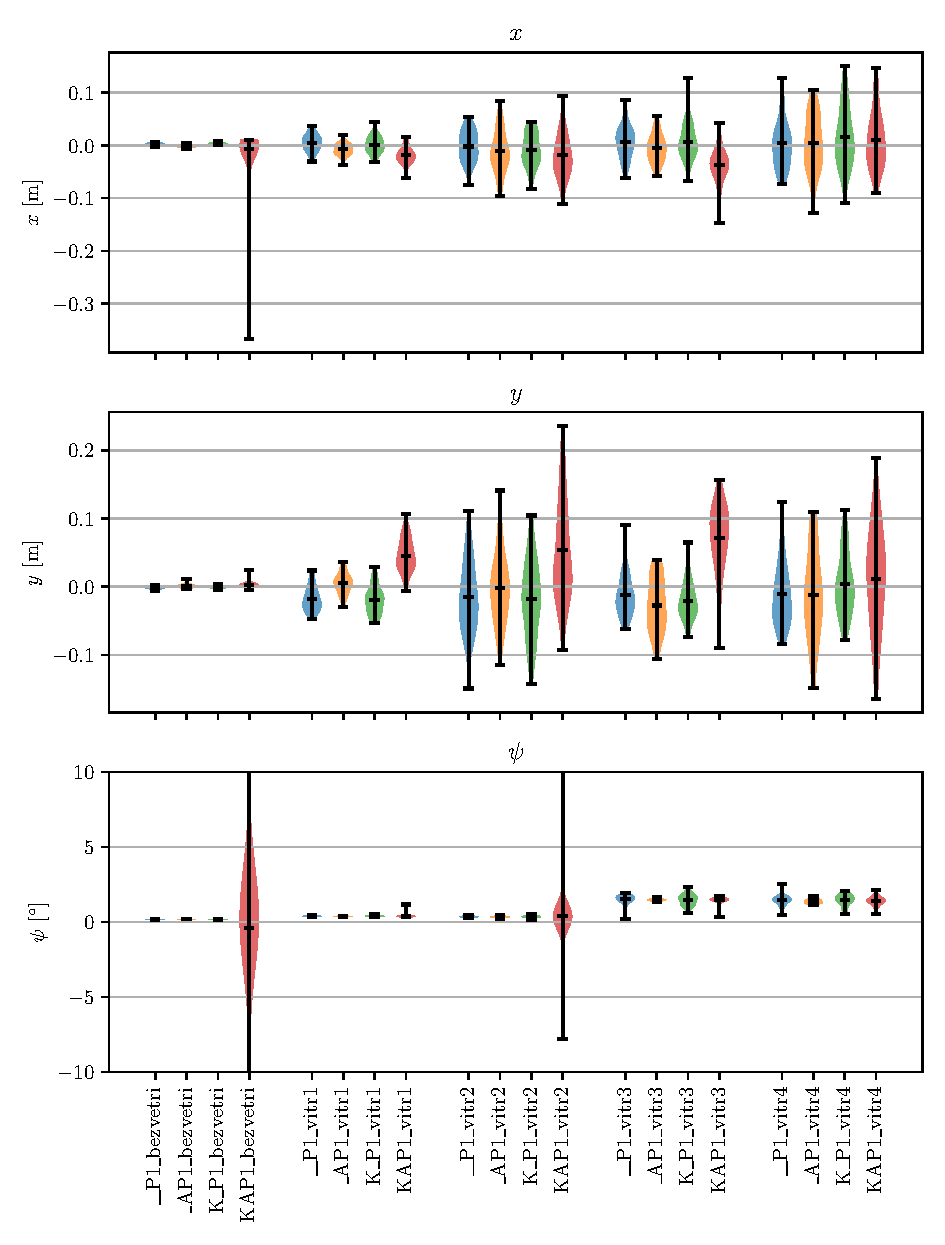
\includegraphics[width=0.9\textwidth]{img/results/presnostDotyku.pdf}
      \caption[Chyba před dosednutím]{Chyba polohy a rotace letadla před požadavkem na dosednutí v~závislosti na použité metodě přistávání a třídě větru. Metody jsou označené barevně a třídy větru jsou od sebe odděleny prostorově. Každý graf zobrazuje střední hodnotu, oba extrémy a odhad rozdělení dané chyby.}
      \label{fig:dosednutiViolin}
    \end{figure}

    Před dosednutím je odchylka polohy od plošiny v~případě všech algoritmů kromě KAP (odhad polohy s~Kálmánovým filtrem přistávající po skloněné přímce) podobná a to v~řádu nižších jednotek centimetrů v~obou prostorových souřadnicích, kdy nejhorší je s~průměrnou odchylkou \mistoPredPristaniYmeanLAPILvitrIII~m metoda přistávající po skloněné přímce bez Kálmánova filtru v~případě čerstvého větru v~souřadnici $y$. Metoda KAP tuto mez překračuje ve 4 případech, přičemž nejhorší je za čerstvého větru s~výchylkou \mistoPredPristaniYmeanKAPILvitrIII~m. Průměrná odchylka v~úhlu natočení $\psi$ je až na výjimky u~metody KAP za bezvětří a při mírném větru s~poryvy nízká do přibližně 2$^\circ$. Se sílícím větrem a poryvy tato odchylka roste a mezi jednotlivými pokusy jsou větší rozdíly. V~prostorových souřadnicích je patrný vliv rychlosti větru i poryvů zejména na rozdíly mezi pokusy, vliv na samotnou odchylku nelze odlišit od šumu.

    \begin{figure}[H]
      \centering
      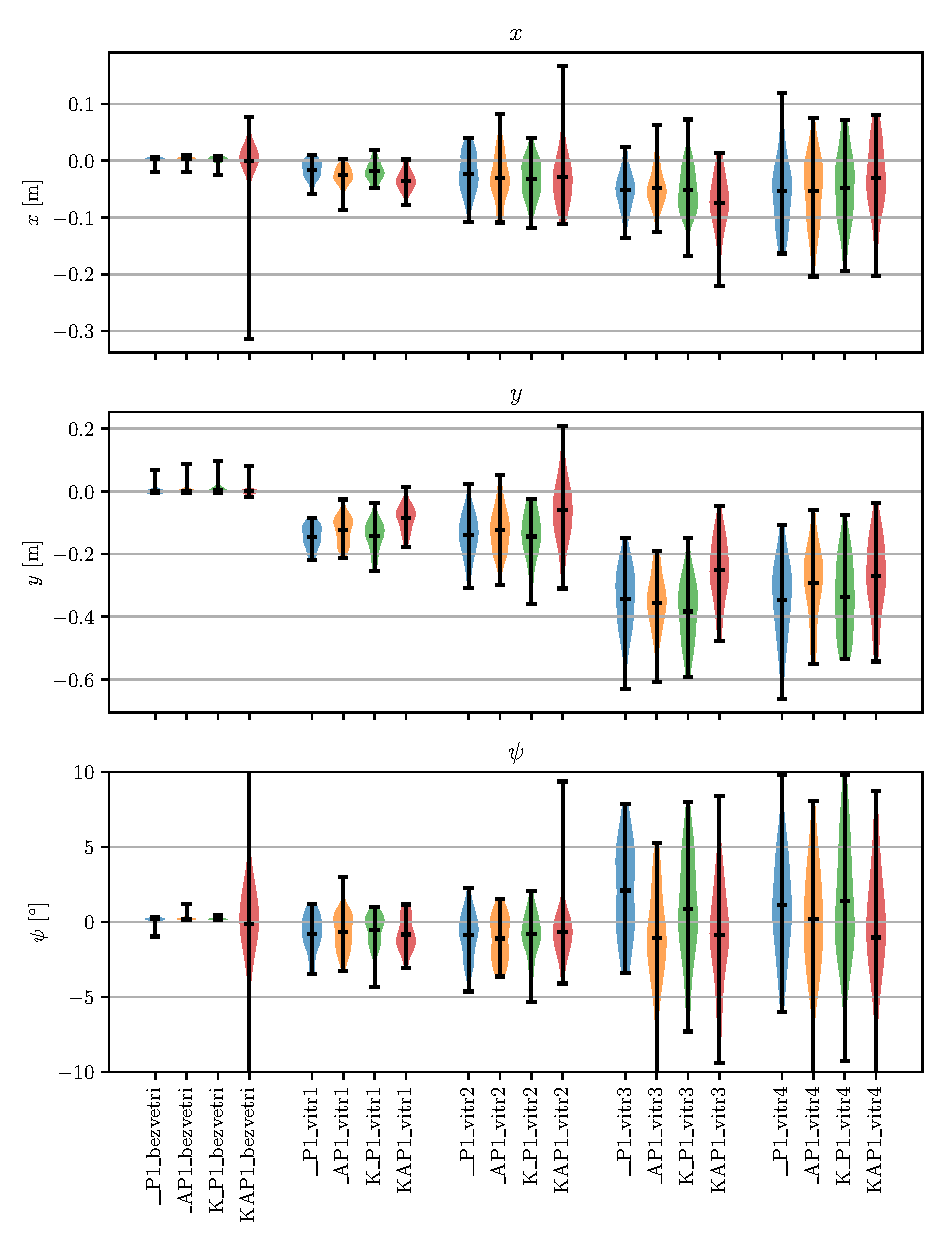
\includegraphics[width=0.9\textwidth]{img/results/presnostPristani.pdf}
      \caption[Chyba přistání]{Chyba polohy a rotace letadla po jeho uvedení do klidu v~závislosti na použité metodě přistávání a třídě větru. Metody jsou označené barevně a třídy větru jsou od sebe odděleny prostorově. Každý graf zobrazuje střední hodnotu, oba extrémy a odhad rozdělení dané chyby.}
      \label{fig:pristaniViolin}
    \end{figure}

    Odchylky po uvedení letadla do klidu jsou výrazně větší, protože tření mezi plošinou a letadlem není po dotyku dostatečné ani při nastavení vysokého koeficientu tření obou ploch v~simulátoru a při doběhu motorů před deaktivací je letadlo snášeno ve směru větru po plošině. Výsledkem je zvyšující se polohová odchylka v~1 směru pro rostoucí rychlost větru patrná u~všech metod přistávání. Pro úhlovou odchylku platí zvětšování rozdílů mezi jednotlivými případy přistávání, ale posun v~jednom směru není příliš patrný. Výsledky všech metod jsou srovnatelné, ale metody, které využívají skloněnou trajektorii (\_AP a KAP) mají ve většině případů průměrnou odchylku bližší 0 než ostatní metody, jeden takový případ ukazuje i \cref{fig:presnostPristani}.

    \begin{figure}
      \centering
      \begin{subfigure}[b]{0.495\textwidth}
        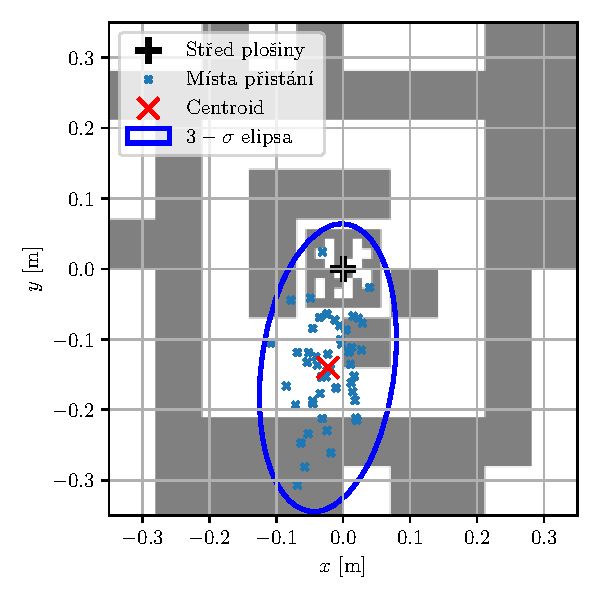
\includegraphics[width=\textwidth]{img/results/__P1_vitr2_pristani.pdf}
        \caption{\_\_P, mírný s~poryvy}
      \end{subfigure}
      \hfill
      \begin{subfigure}[b]{0.495\textwidth}
        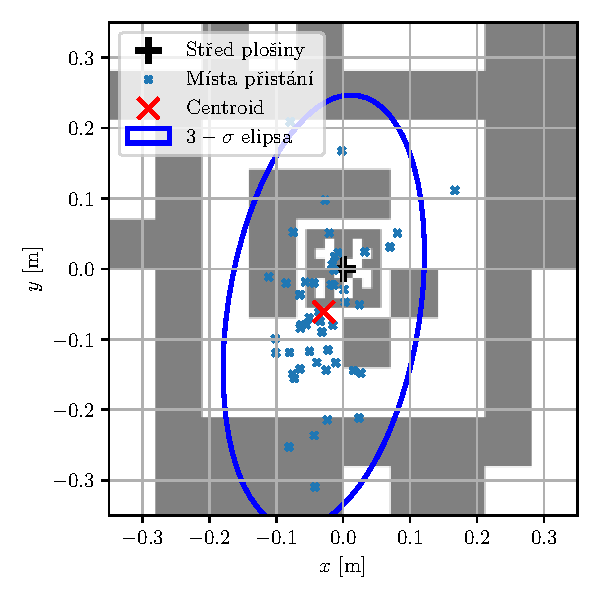
\includegraphics[width=\textwidth]{img/results/KAP1_vitr2_pristani.pdf}
        \caption{KAP, mírný s~poryvy}
      \end{subfigure}
      \caption[Příklad porovnání přistání]{Porovnání míst přistání, jejich centroidů a kovariančních elips pro dva příklady algoritmů za mírného větru.}
      \label{fig:presnostPristani}
    \end{figure}
  
  \section{Přesnost přistávání} \label{sec:presnostPristavani}
    Další experiment zjišťoval přesnost celého přistávacího manévru, kdy během každé ze simulací postupně počítal střední absolutní chybu (\acrshort{mae}) v~souřadnicích $x, y$ a rotaci $\psi$ v~každém kroku algoritmu vůči jím požadované trajektorii (ve 2 případech přímka kolmo procházející středem plošiny, ve 2 případech skloněná přímka pod stejným úhlem jako v~daném větru přistávající dron nasměrovaná proti němu). Stejně jako minulý experiment byl tento pokus proveden 50x pro každý prvek kartézského součinu metody přistávání $\times$ třídy větru. \Cref{tab:mae} shrnuje \acrshort{mae} na konci přistávání pro dané podmínky simulace.

    \begin{table}
      \centering
      \begin{tabular}{@{}lllllll@{}}
    \hline
alg.                 &        & bezvětří              & slabý                  & slabý s p.          & čerstvý      & čerstvý s p. \\\hline
\multirow{3}{*}{\_\_P} & $x$    & \MAExLLPILbezvetri   & \MAExLLPILvitrI         & \MAExLLPILvitrII & \MAExLLPILvitrIII & \MAExLLPILvitrIV \\
                     & $y$    & \MAEyLLPILbezvetri   & \MAEyLLPILvitrI         & \MAEyLLPILvitrII & \MAEyLLPILvitrIII & \MAEyLLPILvitrIV \\
                     & $\psi$ & \MAEyawLLPILbezvetri & \MAEyawLLPILvitrI       & \MAEyawLLPILvitrII & \MAEyawLLPILvitrIII & \MAEyawLLPILvitrIV \\\multicolumn{7}{l}{}\\
\multirow{3}{*}{\_AP} & $x$    & \MAExLAPILbezvetri   & \MAExLAPILvitrI         & \MAExLAPILvitrII & \MAExLAPILvitrIII & \MAExLAPILvitrIV \\
                     & $y$    & \MAEyLAPILbezvetri   & \MAEyLAPILvitrI         & \MAEyLAPILvitrII & \MAEyLAPILvitrIII & \MAEyLAPILvitrIV \\
                     & $\psi$ & \MAEyawLAPILbezvetri & \MAEyawLAPILvitrI       & \MAEyawLAPILvitrII & \MAEyawLAPILvitrIII & \MAEyawLAPILvitrIV \\\multicolumn{7}{l}{}\\
\multirow{3}{*}{K\_P} & $x$    & \MAExKLPILbezvetri   & \MAExKLPILvitrI         & \MAExKLPILvitrII & \MAExKLPILvitrIII & \MAExKLPILvitrIV \\
                     & $y$    & \MAEyKLPILbezvetri   & \MAEyKLPILvitrI         & \MAEyKLPILvitrII & \MAEyKLPILvitrIII & \MAEyKLPILvitrIV \\
                     & $\psi$ & \MAEyawKLPILbezvetri & \MAEyawKLPILvitrI       & \MAEyawKLPILvitrII & \MAEyawKLPILvitrIII & \MAEyawKLPILvitrIV \\\multicolumn{7}{l}{}\\
\multirow{3}{*}{KAP} & $x$    & \MAExKAPILbezvetri   & \MAExKAPILvitrI         & \MAExKAPILvitrII & \MAExKAPILvitrIII & \MAExKAPILvitrIV \\
                     & $y$    & \MAEyKAPILbezvetri   & \MAEyKAPILvitrI         & \MAEyKAPILvitrII & \MAEyKAPILvitrIII & \MAEyKAPILvitrIV \\
                     & $\psi$ & \MAEyawKAPILbezvetri   & \MAEyawKAPILvitrI         & \MAEyawKAPILvitrII & \MAEyawKAPILvitrIII & \MAEyawKAPILvitrIV \\\hline
\end{tabular}%
      \caption[Střední absolutní chyba přistávání]{Střední absolutní chyba sledování požadované trajektorie v~závislosti na větrných podmínkách a použitém algoritmu. K~v~názvu algoritmu znamená, že byl použit Kálmánův filtr, A~znamená přistání po skloněné přímce a P proporcionální regulátor rychlosti.}
      \label{tab:mae}
    \end{table}

    Na přesnost přistávání má negativní vliv rychlost větru i jeho nárazy, kvůli zvolenému směru jsou hlavní projevy patrné v~ose $y$. Algoritmy bez Kálmánova filtru (\_\_P a \_AP) si při slabém větru bez poryvů vedou lépe než ty s~Kálmánovým filtrem, zatímco při silnějším větru mají menší \acrshort{mae} metody se skloněnou trajektorií (\_AP a \_KAP), na jejichž \acrshort{mae} nemá zvyšující se intenzita větru tak velký vliv. V~rotaci jsou vždy lepší algoritmy bez Kálmánova filtru a zdá se, že poryvy větru mají navzdory očekávání spíše pozitivní vliv na střední chybu rotace. Kromě zmíněných odlišností jsou výsledky jednotlivých algoritmů obecně srovnatelné.
  \section{Úspěšnost přistávání} \label{sec:uspesnost}
    Během silných poryvů se stává, že se letoun v~blízkosti plošiny vychýlí natolik, že se marker na plošině dostane mimo zorné pole kamery. V~takový okamžik ztrácí algoritmus možnost podle obrazu odhadovat vzájemnou polohu \acrshort{uav} a značky, proto čeká 50 snímků s~požadavkem na fixní polohu na případné odregulování poruchy způsobené poryvem, po kterém by mohl být marker opět viditelný, a mezitím stoupá rychlostí 0{,}3~m/s. {Neobjeví-li} se během této doby, považuje se pokus o~dosednutí za neúspěšný a je opakován tak, že dron podle \acrshort{gps} přelétává na přibližnou polohu plošiny do výšky 10~m a sleduje, jestli se objeví na snímcích z~kamery marker. Po úspěšné detekci se opět pokouší přistát. Při tomto experimentu se zaznamenával počet pokusů o~dosednutí a vypočetla se jeho střední hodnota přes 50 provedených pokusů u~všech dvojic metod přistávání a tříd větru. Výsledky jsou v~\refskl{tab:uspesnost}{tabulce}.

    \begin{table}[H]
      \centering
      \begin{tabular}{@{}llllll@{}}
    \hline
alg.  & bezvětří                           & slabý                                & slabý s p.                      & čerstvý                        & čerstvý s p. \\\hline
\_\_P & \landingRetriesMeanLLPILbezvetri   & \landingRetriesMeanLLPILvitrI         & \landingRetriesMeanLLPILvitrII & \landingRetriesMeanLLPILvitrIII & \landingRetriesMeanLLPILvitrIV  \\
\_AP & \landingRetriesMeanLAPILbezvetri   & \landingRetriesMeanLAPILvitrI         & \landingRetriesMeanLAPILvitrII & \landingRetriesMeanLAPILvitrIII & \landingRetriesMeanLAPILvitrIV \\
K\_P & \landingRetriesMeanKLPILbezvetri   & \landingRetriesMeanKLPILvitrI         & \landingRetriesMeanKLPILvitrII & \landingRetriesMeanKLPILvitrIII & \landingRetriesMeanKLPILvitrIV \\
KAP & \landingRetriesMeanKAPILbezvetri   & \landingRetriesMeanKAPILvitrI         & \landingRetriesMeanKAPILvitrII & \landingRetriesMeanKAPILvitrIII & \landingRetriesMeanKAPILvitrIV \\\hline
\end{tabular}%
      \caption[Úspěšnost přistávání]{Úspěšnost přistávání vyhodnocená jako průměrný počet pokusů potřebných k~úspěšnému dosednutí v~závislosti na větrných podmínkách a použítém algoritmu.}
      \label{tab:uspesnost}
    \end{table}

    Úspěšnost přistávání se liší až při čerstvém větru, kde ji vylepšuje sklonění trajektorie i Kálmánův filtr tím, že snižují průměrný potřebný počet pokusů o~dosednutí. Při použití obou strategií je průměrný počet pokusů mírně vyšší než kdyby se Kálmánův filtr nepoužil.

  \section{Doba trvání přistávání}
    Doba, za jak dlouho \acrshort{uav} přistane souvisí s~úspěšností přistávání, protože při opakováném hlednání plošiny se ztrácí čas, a také s~přesností, jelikož rychlost klesání roste s~klesající odchylkou od požadované dráhy. Vyhodnocovaná doba se počítala od okamžiku nalezení fiduciárního markeru v~obrazu do okamžiku uvedení letadla do klidu a i v~tomto případě bylo provedeno stejných 50 opakování pro každou z~20 dvojic podmínek. Střední hodnota, extrémy a odhad rozdělení pro všechny možnosti přes všechna jejich opakování je v~grafu na \refskl{fig:dobaPristavani}{obrázku}.

    \begin{figure}[H]
      \centering
      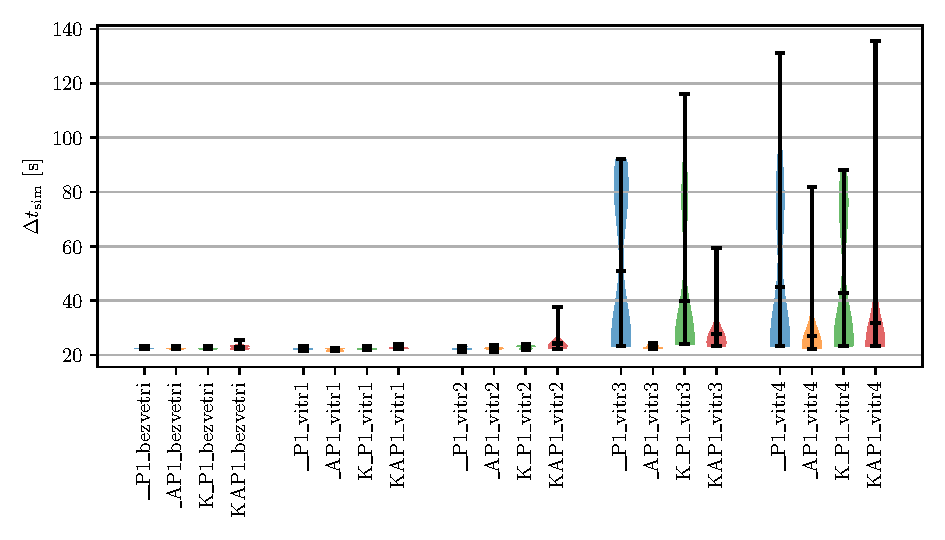
\includegraphics[width=\textwidth]{img/results/trvani.pdf}
      \caption[Doba trvání přistávání]{Doba trvání přistávání od jeho zahájení po uvedení letadla do klidu. Pro každou z~kombinací algoritmu (každý má přiřazenou barvu) a třídy větru (skupiny na vodorovné ose) je vyznačena střední hodnota doby trvání, extrémy a odhad jejího rozdělení.}
      \label{fig:dobaPristavani}
    \end{figure}

    Ve výsledcích je patrné snížení průměru doby přistávání u~metody se skloněnou trajektorií bez Kálmánova filtru a za většího větru i u~obou metod s~Kálmánovým filtrem, jak bylo očekáváno dle průměrného počtu pokusů o~přistání (\refskl{sec:uspesnost}{podkapitola}), pokusy jsou také patrné v~rozdělení časů v~grafu (\cref{fig:dobaPristavani}). Metody s~Kálmánovým filtrem za mírného větru přistávají průměrně pomaleji, za čerstvého větru a bezvětří jsou lepší než základní metoda a mají za čerstvého větru mají lepší rozdělení časů napříč pokusy, jež je koncentrováno více v~nižších hodnotách.
    

  \section{Střední doba výpočtu v~jednom kroku algoritmu} \label{sec:stredniDobaVypoctu}
    Pro posouzení výpočetní náročnosti jednotlivých metod byla v~průběhu přistávání zaznamenávána také průměrná doba potřebná k~výpočtu jednoho kroku algoritmu od obdržení snímku z~kamery po předání řídicího požadavku letové řídicí jednotce. Krok algoritmu zahrnuje detekci fiduciárních markerů, odhad jejich polohy, přepočet polohy do vodorovné souřadné soustavy dronu, volitelně filtraci Kálmánovým filtrem, přepočet na odchylku od vybrané trajektorie a výpočet požadavku na rychlosti v~jednotlivých osách letadla pomocí PID regulátorů. Průměrná (přes pokusy) střední (přes jednotlivé kroky během přistávání) doba výpočtu jednoho kroku přistávacího algoritmu je pro dané metody uvedena v~\refskl{tab:dobaKroku}{tabulce}.

    \begin{table}
      \centering
      \begin{tabular}{@{}ll@{}}
    \hline
alg.  & průměr [s] \\\hline
\_\_P &$ 1{,}44  \times 10^{-2}$\\
\_AP &$ 1{,}48  \times 10^{-2}$\\
K\_P &$ 2{,}47  \times 10^{-2}$\\
KAP &$ 2{,}95  \times 10^{-2}$\\\hline
\end{tabular}%
      \caption[Průměrná střední doba jednoho kroku algoritmu]{Průměrná střední doba jednoho kroku přistávacího algoritmu vážená počtem kroků během pokusu.}
      \label{tab:dobaKroku}
    \end{table}

    Se složitostí algoritmu roste i čas potřebný k~provedení jednoho jeho kroku, při sklonění trajektorie se krok oproti základnímu algoritmu zpomalí o~0{,}4~ms, při použití Kálmánova filtru je nárůst asi $2/3$ a využijí-li se obě možnosti, čas potřebný k~výpočtu naroste o~$15{,}1$~ms na více než dvojnásobek.
  \section{Vliv stínu na podíl nedetekovaných markerů} \label{sec:stin}
    
  % \section{Ověření nezávislosti výsledků na směru větru}
  %   Aby se ušetřil počet pokusů, ověřil bych jen za silného větru, zda se nějak liší průběh přistávání.
  % \section{Ověření nezávislosti výsledků na vzájemné počáteční poloze dronu a plošiny}
  % \section{Odhad kovariančních matic pro Kálmánův filtr}
  %   Nevím, jestli vůbec podrobněji rozepisovat zde, když už je to popsáno v \refskl{sec:kalmanoffboardpid}{podkapitole}.